\documentclass{article}
\usepackage{graphicx} 
\usepackage{amssymb}
\usepackage{braket}
\usepackage{hyperref}
\usepackage{braket}
\usepackage{amsmath}


\title{Semester 2 Notes}
\author{Connor Stocks}

\newtheorem{theorem}{Theorem}


\begin{document}

\newcounter{eq}[section]
\newcommand{\equationref}{\stepcounter{eq}\arabic{section}.\arabic{eq}}
\newcommand{\tagequation}[1]{\[\tag{\equationref}#1\]}

\hypersetup{
    colorlinks,
    citecolor=black,
    filecolor=black,
    linkcolor=black,
    urlcolor=black
}

\maketitle

\newpage
\tableofcontents


\newpage
\section{Analysis II}
\subsection{Propositional Logic}
\marginpar{27/1/25}




\begin{itemize}
    \item \(\lnot(p\cup q) = (\lnot p)\cap(\lnot q)\)
    \item \(\lnot(p\cap q) = (\lnot p)\cup(\lnot q)\)
    \item \(\lnot(\exists p) = \forall p\)
    \item \(p \Rightarrow q = (p\cap q)\cup \lnot q\)
    \item so \(\lnot (p\Rightarrow q) = (\lnot p \cup\lnot q)\cap \lnot\lnot q = \lnot p\cup q\)
\end{itemize}

\subsection{Continuous Functions}
\marginpar{31/1/25}

\subsubsection*{Continuity}

\begin{itemize}
    \item For \(f: D\rightarrow\mathbb{R}\), f is continuous at a point \(a\in D\) if:
    \\\(\forall\epsilon>0, \exists\delta>0:\forall x\in D, |x-a|<\delta\Rightarrow|f(x)-f(a)|<\epsilon\)
    \item f is uniformly coninuous if continuous \(\forall a\), or
    \marginpar{3/2/25}
    \\\(\forall\epsilon>0, \exists\delta>0:\forall x, y\in D, |x-y|<\delta\Rightarrow|f(x)-f(y)|<\epsilon\)
    \item In general, continuity \(\not\Rightarrow\) uniform continuity

    \item A function \(f:D\rightarrow\mathbb{R}\) is continuous at \(a\in\mathbb{R}\) iff:
    \\\(\forall(x_n)_{n\in\mathbb{N}}, x_n\in D, \lim_{n\to\infty}{x_n} = a, \lim_{n\to\infty}{f(x_n)}=f(a)\)
\end{itemize}


\begin{theorem}[Intermediate Value Theorem]

    for \(f:D\rightarrow C\subseteq\mathbb{R}\)

    then \(u\in C\Rightarrow \exists x\in D: u=f(x)\)

\end{theorem} 


\newpage
\section{waves and fields}
\subsection{Periodic Motion}
\subsubsection*{Periodic Motion In 1D}
\marginpar{28/1/25}

\begin{itemize}
    \item Periodic motion is one in which the position repeats values regularly
    \item It can be characterised like so:
    \begin{itemize}
        \item[] \(r(t + nT) = r(t), \forall t\in\mathbb{R}, n\in\mathbb{N}, T=period\)
    \end{itemize}
    \item If we consider a situation in a consevative field, with a potential \(u(x)\), and a system with a total energy E:

    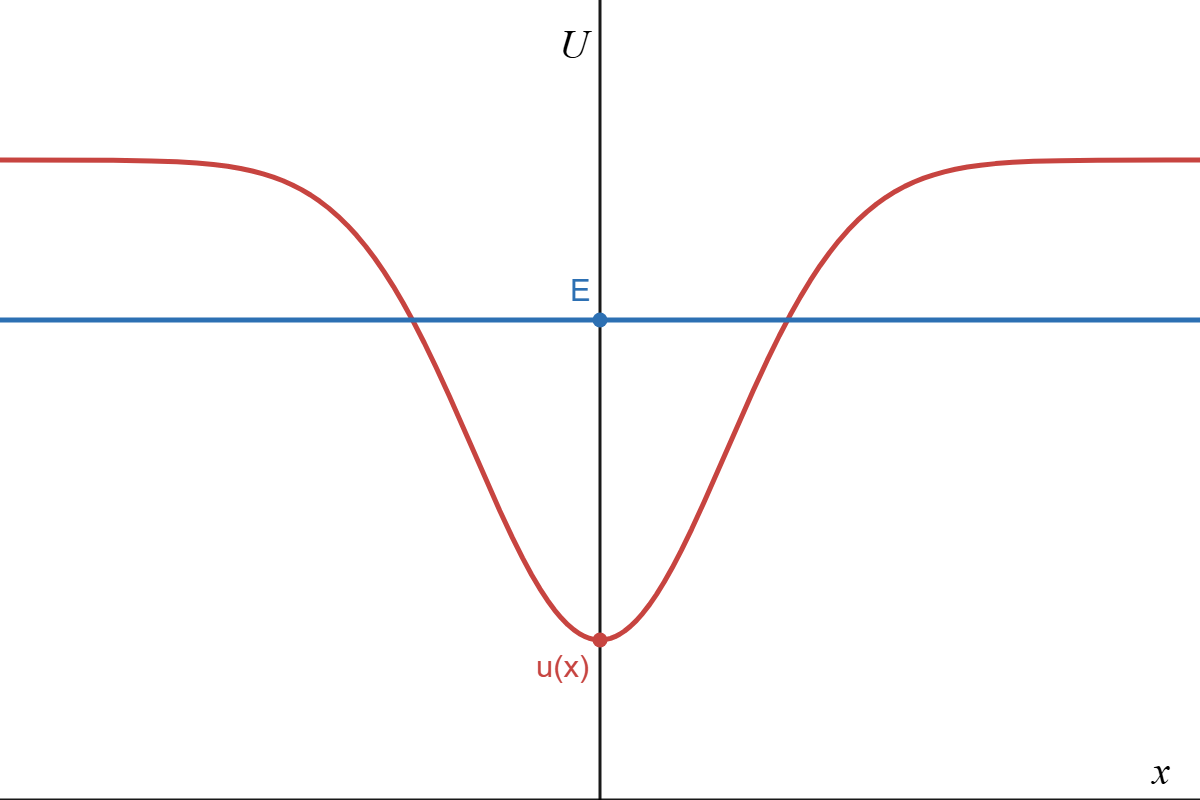
\includegraphics[width = 0.5\linewidth]{year1/wfmp/periodic-motion/potential-without-bounds.png}

    \item We can see that the system would be bound within the region $U < E$: 

    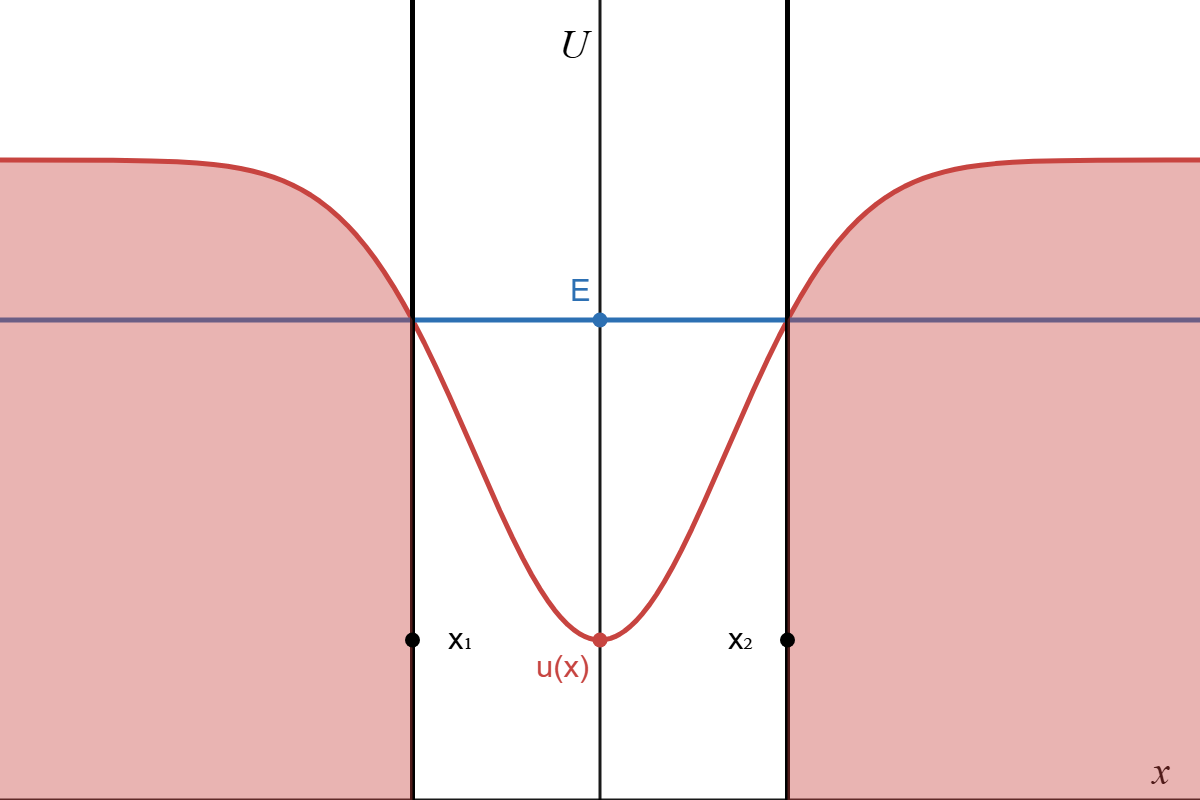
\includegraphics[width = 0.5\linewidth]{year1/wfmp/periodic-motion/potential-with-bounds.png}

    \item This naturally leads to periodic motion, as at \(x = x_1, v = 0\)
    \item At this point, the energy is not minimised, and so the system tends towards \(x = 0\), 
    where \(v \not= 0\), causing periodic motion. 
    
    \marginpar{30/1/25}

    \item One way to achieve this is through simple harmonic motion (SHM)
    \item SHM is any system where \(\ddot x = -x\)
    \item We can see here that \(u(x) = -\int f dx = \int\frac{\ddot x}{m}dx\), 
    or \(f = -\frac{du}{dx} \Rightarrow m\ddot x = -\frac{du}{dx}\)
    \item We can then add another term to take energy out of the system:
    \item \(m\ddot x = -\frac{du}{dx} - \gamma\dot x\) in general. 
    \item This describes a frictional force, causing damped harmonic motion (DHM)
    \item This will lead to the energy gradually decreasing:
    
    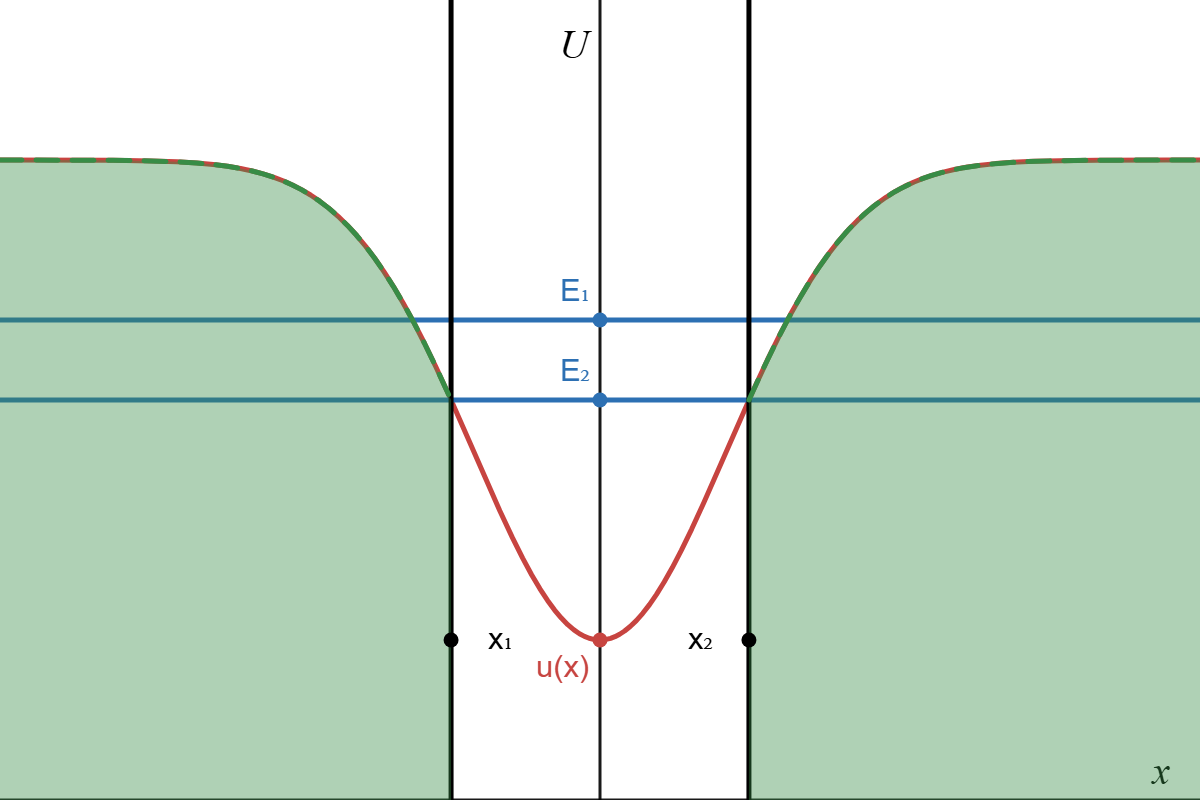
\includegraphics[width = 0.5\textwidth]
    {year1/wfmp/periodic-motion/potential-with-smaller-bounds.png}

    \item Which will result in the following motion:

    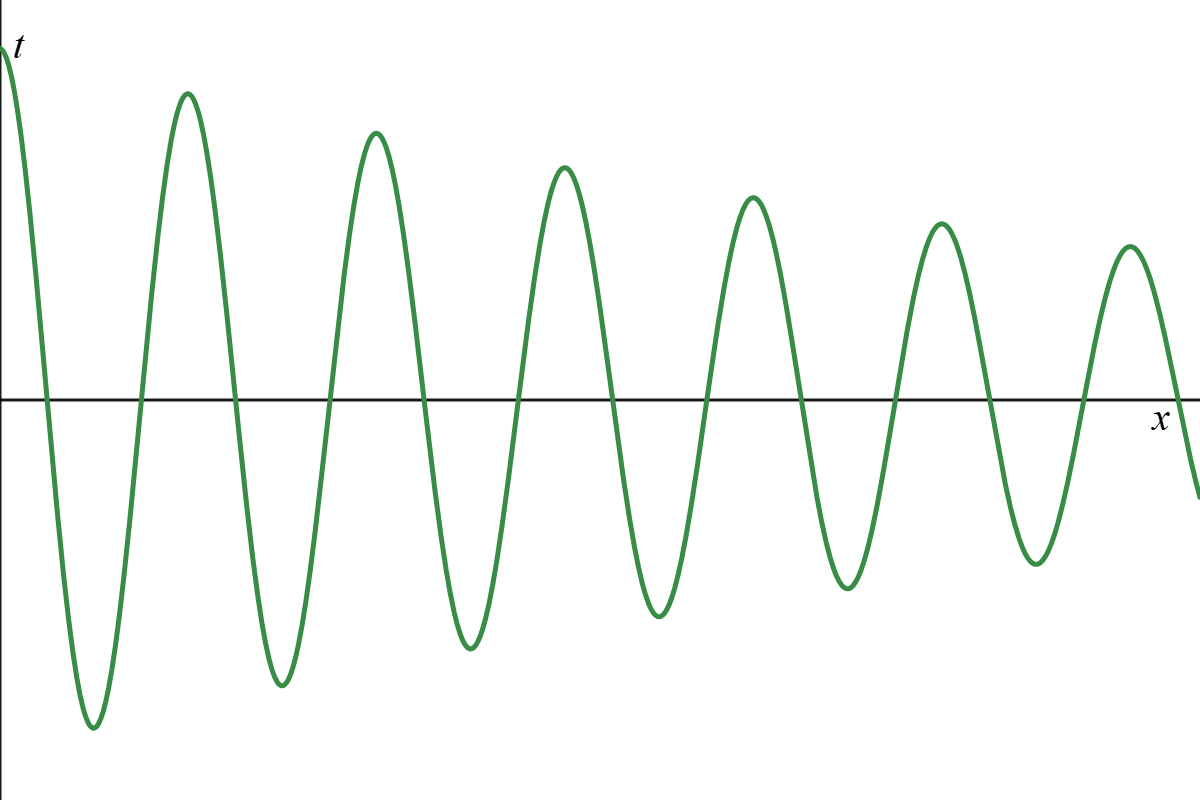
\includegraphics[width = 0.5\textwidth]{year1/wfmp/periodic-motion/DHM.png}
\end{itemize}

\subsubsection*{Periodic Motion In 3D}

\begin{itemize}
    \item Gravity is a conservative force so \(u = u(\vec r)\), and angular momentum is conserved
    \item Evidently, from \(\vec L = \vec r\times\vec p\), the position \(\vec r\) is perpendicular to the constant angular momentum \(\vec L\), and thus the system is confined to a single plane.
    \item Let \(v_{\phi}=\)the component of \(v\) perpendicular to $\vec r$, and \(v_r=\) the component of v parallel to \(\vec r\)
    \item Then \(L=m\vec r\times(r\dot\phi)\)
    \item Since \(K=\frac{1}{2}m\dot{\vec r} = \frac{1}{2}m(\dot{\vec r_{\phi}}^2 +\dot{\vec r_r}^2)=\frac{1}{2}m(\dot r ^2 + r^2\dot\phi ^2)\)
    \item \(\dot\phi = \frac{L}{mr^2} \Rightarrow K = \frac{1}{2}m(\dot r ^2 + r^2(\frac{L}{mr^2})^2)\)
    \item So \(E = K + u = \frac{1}{2}m(\dot r^2 + (L/mr)^2 + u(\vec r))\)
    
\end{itemize}

\subsubsection*{Simple Harmonic Motion}
\marginpar{31/1/25}

\begin{itemize}
    \item Simple harmonic motion is any motion of the form \(x(t) = Acos(\omega t + \phi)\)
    \item From this, we can see that \(\ddot x(t) = -A\omega^2\cos(\omega t+\varphi) = -\omega^2x\)
    \item This differential equation, \(\ddot x \propto x\), characterises simple harmonic oscillation(SHO)
    \item Then, \(f =m\ddot x = -m\omega^2x\), is only dependant on position
    \item Then, the potential energy: \(U(x) = -\int f dx = m\omega^2\int x dx=\frac{1}{2}m\omega^2x^2\)
    \item Then, \(E = K + U = \frac{1}{2}m\dot{x^2} + \frac{1}{2}m\omega^2x^2 = \frac{1}{2}mA^2\omega^2\)
    \item E, K, and U will look like this over time, with \(\overline{U} = \overline{K}\) over one period:
    
    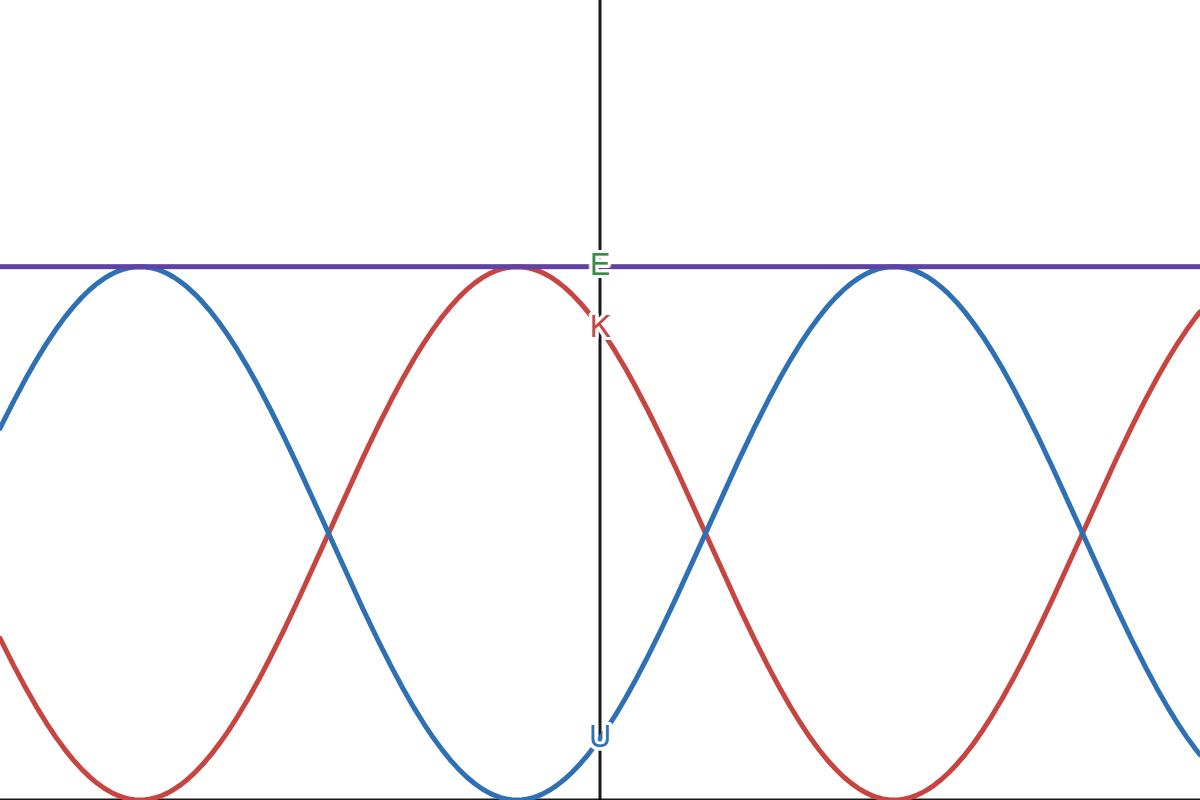
\includegraphics[width = 0.5\linewidth]{year1/wfmp/periodic-motion/osciltor-energy.png}
\end{itemize}


\subsubsection*{Simple Pendulums and Small oscillators}

\begin{itemize}
    \item For a simple pendulum, \(|\tau|=I\ddot{\theta}=-f_{\perp}\cdot r = -f_g\sin(\theta)\cdot l\)
    \item Then, using the small angle approximation \(\sin(\theta) = \theta\):
    
    \(I\ddot{\theta}=-f_g l\theta\)
 
    \item Another example of simphe harmonic motion is the torsion pendulum
    \item This is a mass on a string that can twist around its axis:
    
    \(\tau=-c\theta\Rightarrow I\ddot\theta=-c\theta\)
    
\end{itemize}

\subsubsection*{Damped Harmonic Motion}

\begin{itemize}
    \marginpar{6/2/25}
    \item We expect the amplitude A of a damped harmonic oscillator to decrease over time.
    \item For DHM, The 2nd law of motion looks like this:
    \item \(m\ddot x = -kx - b\dot x\)
    \item Setting b=0, we recover the SHM characteristic equation
    \item For \(b^2-4km<0\), This is called underdamping
    \item Underdamping will have the following form of motion:
    \tagequation{x(t) = Ae^{-\frac{b}{2m}t}\cos(\omega t + \varphi)}
    
    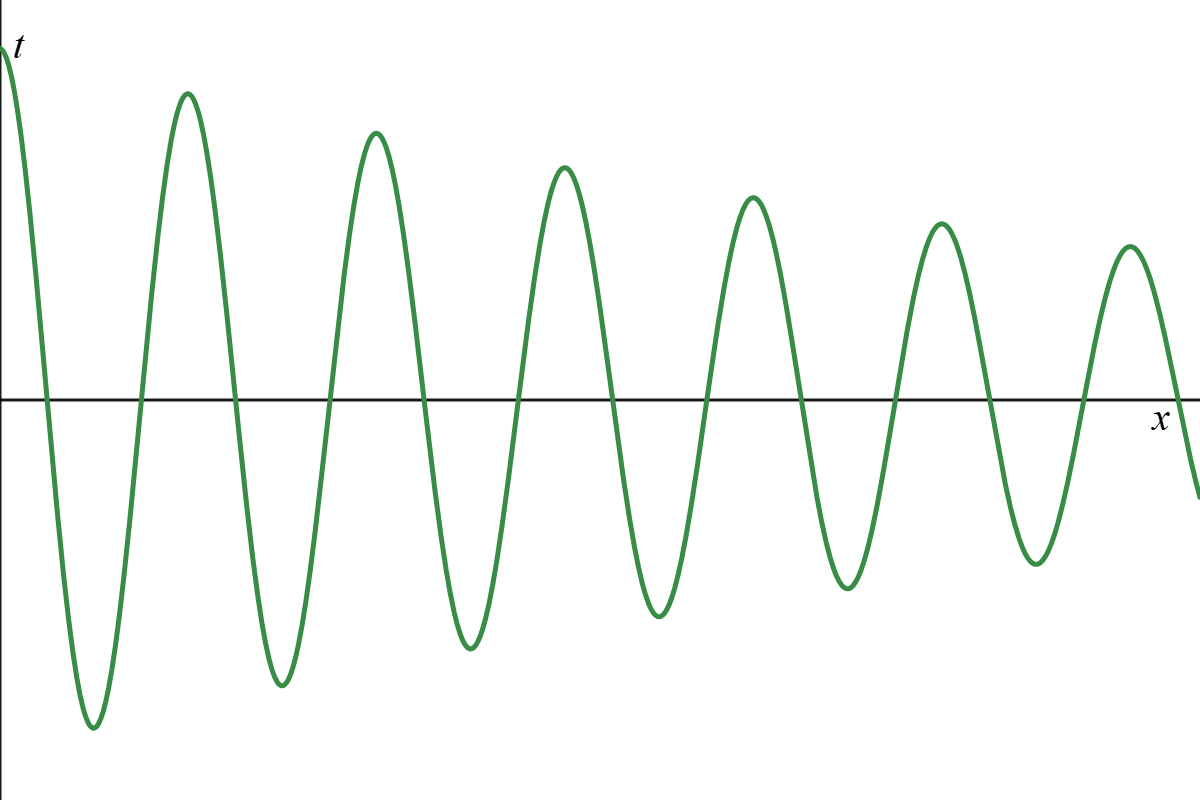
\includegraphics[width = .5\linewidth]{year1/wfmp/periodic-motion/DHM.png}
    \item Then considering the quantity \(\frac{2m}{b}\), we see \(|x(t+\frac{2m}{b})|=e^{-1}|x(t)|\)

    \item If \(b^2>4mk\), we get overdamped motion:
    \item \(x(t)=A_1 e^{-\lambda_1 t} + A_2 e^{-\lambda_2 t}\)

    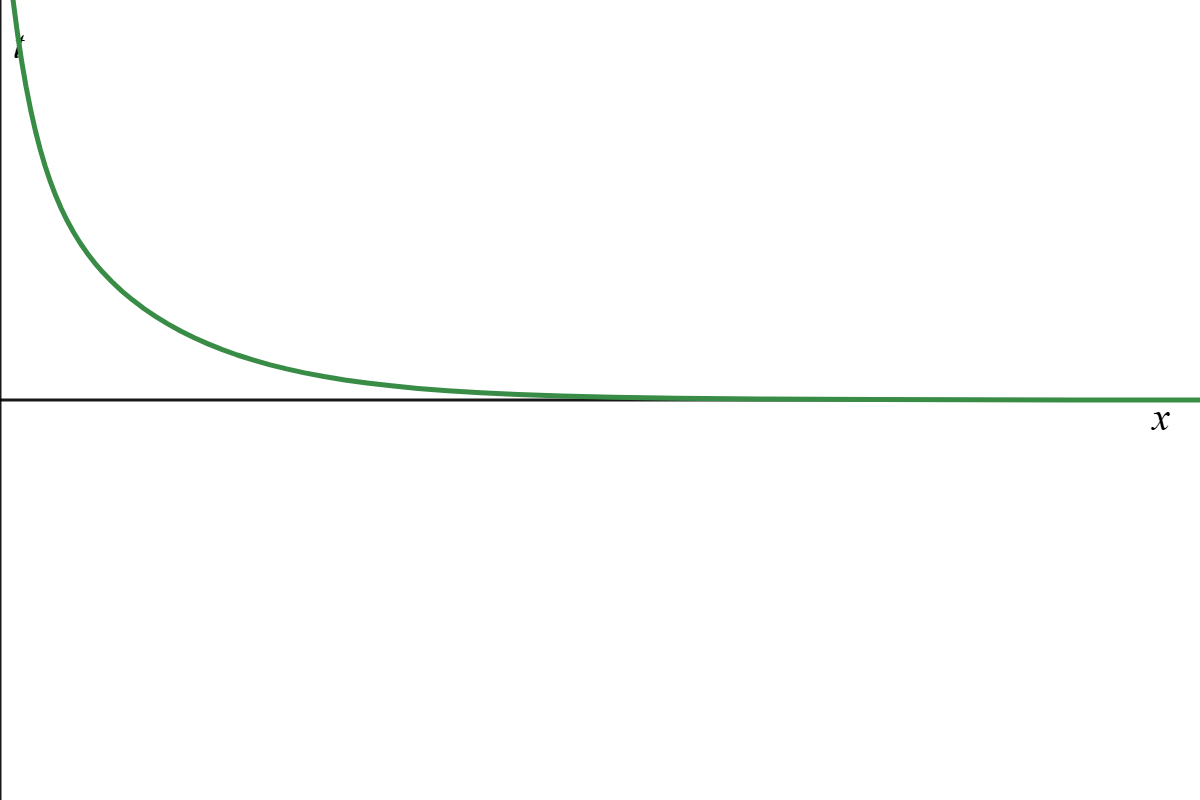
\includegraphics[width=.5\linewidth]{year1/wfmp/periodic-motion/overdamped.png}
    \item and if \(b^2=4mk\), critically damped Motion:
    \item \(x(t)=(A_1 + A_2 t)e^{-\frac{b}{2m}t}\)
    
    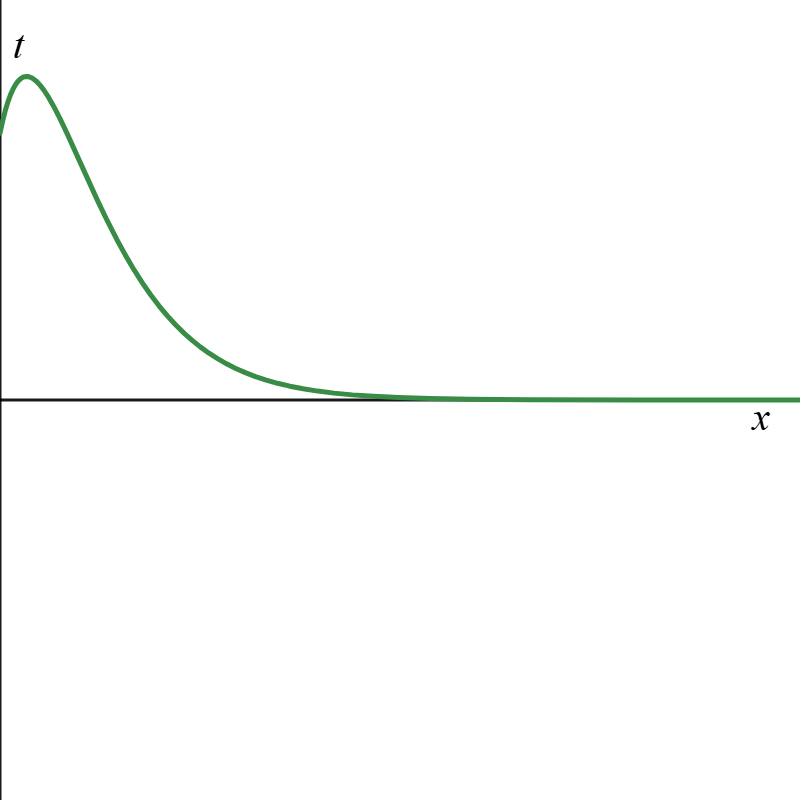
\includegraphics[width=.5\linewidth]{year1/wfmp/periodic-motion/critically damped.png}

\end{itemize}

\subsubsection*{Forced Harmonic Oscillation \& Resonance}

\begin{itemize}
    \marginpar{7/2/25}
    \item A forced harmonic oscillator (FHO) is one subject to an external driving force \(F_d\)
    \item \(\ddot x + \frac{b}{m}\dot x + \frac{k}{m}=\frac{1}{m}F_d\)
    \item If the driving force is also periodic, the motion will oscillate at the driving frequency \(f_d\)
    \tagequation{\omega_r=\omega_0\sqrt{\frac{k}{m}-\frac{b^2}{2m^2}}}
    \item Where A is maximised at \(\omega_d=\omega_r\)
\end{itemize}



\newpage
\section{Modern Physics}
\subsection{Black Body Radiation}

\marginpar{31/1/25}
\subsubsection*{Observations}
\begin{itemize}
    \item Black bodies satisfy 3 criteria:
    \begin{itemize}
        \item absorbs all incident radiation
        \item emits as much radiation as possible at any wavelength
        \item emits radiation isotropically
    \end{itemize}
    \item By studying the spectra of black bodies at different temperatures:
    
    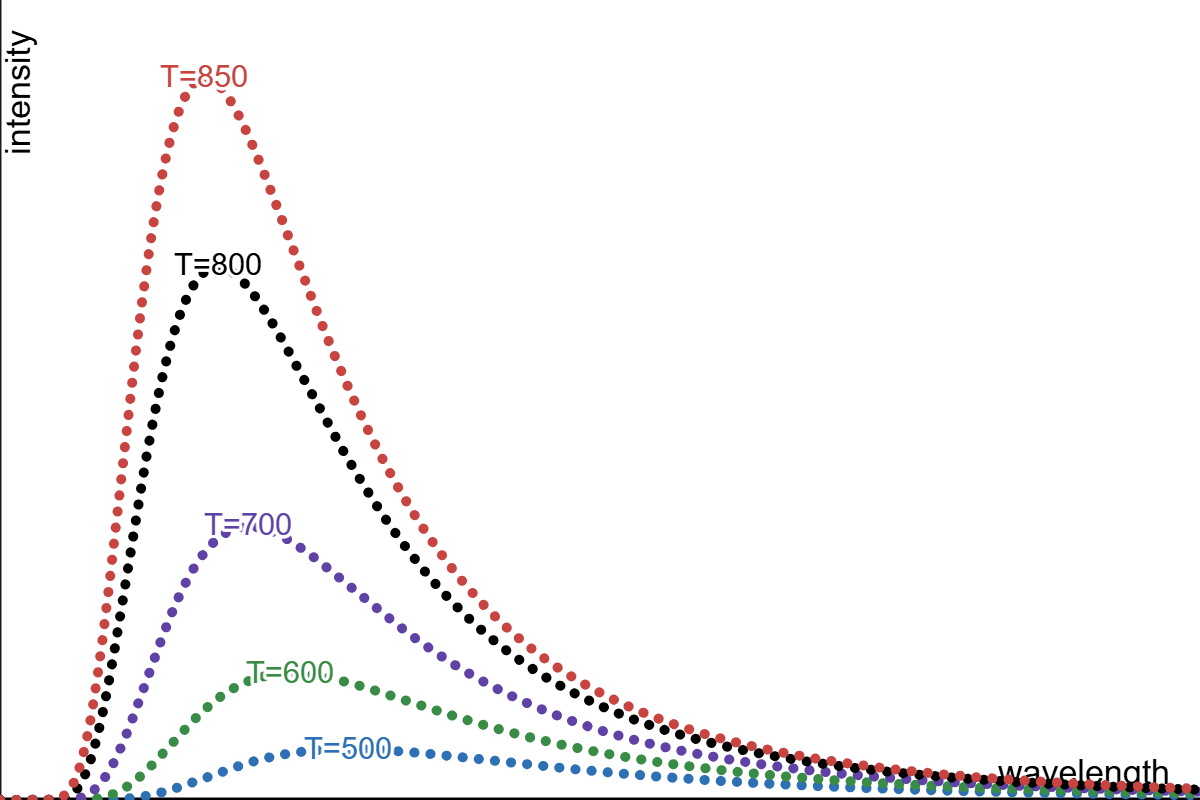
\includegraphics[width=.5\linewidth]{year1/wfmp/black body radiation/blackbody-spectra.png}
    \item We can observe 2 main laws:
    \begin{itemize}
        \item Wein's displacement law: \(\lambda_{max} = \frac{b}{T}\)
        \item Stephans law: \(P(T) = \sigma AT^4\)
    \end{itemize}
\end{itemize}

\subsubsection*{Rayleigh-Jeans Law}

\begin{itemize}
    \item In June 1900, John Rayleigh discovered that the spectral raiance \(\propto \lambda^{-4}\)
    \item In 1905, James Jean derived the full Rayleigh-Jeans law including constants
    \item The Rayleigh-Jeans law is a classical approximation of the radiance of a black body
    \item Rayleigh-Jeans law can be expressed as so:
    \tagequation{B(\lambda, T)=\frac{2ck_b T}{\lambda^4}}
    \item This produced the following prediction for spectral radiance at T=800:
    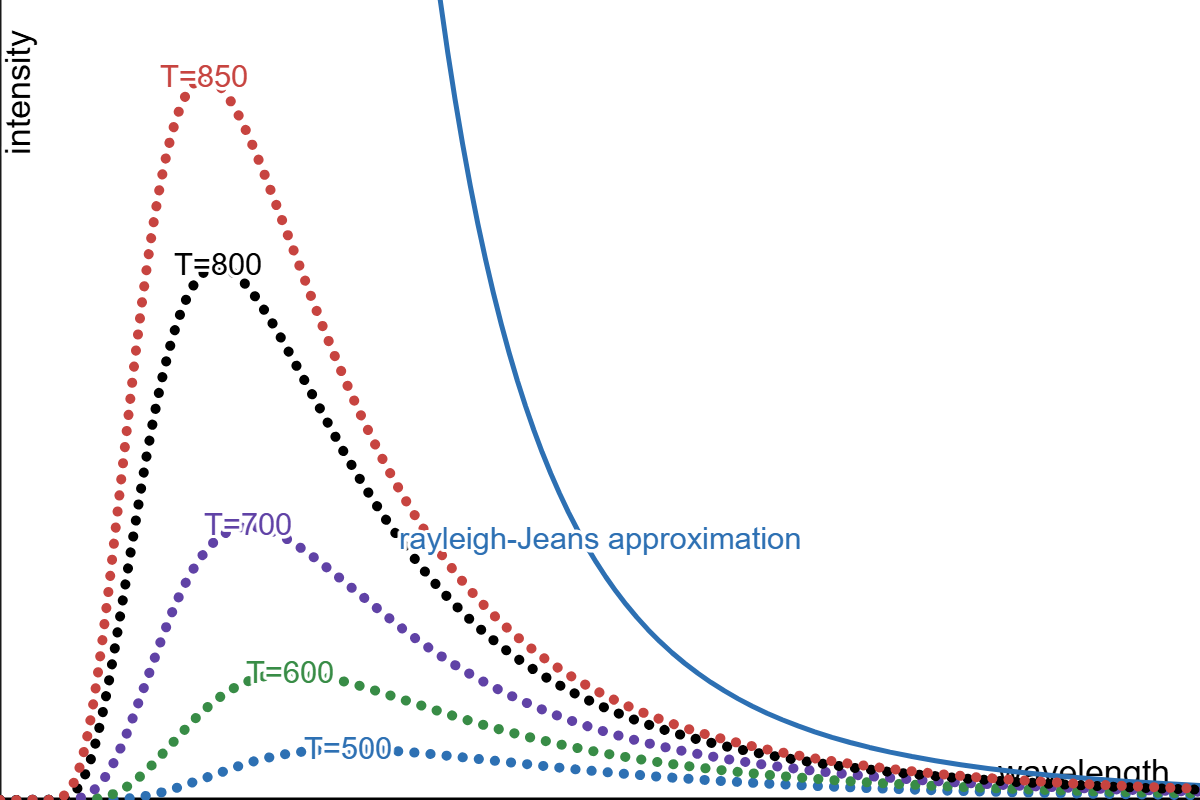
\includegraphics[width=.5\linewidth]{year1/wfmp/black body radiation/r-j-approximation.png}
    \item This presents many problems, mainly that it doesnt match for \(\lambda < \lambda_p\), and \(I\rightarrow\infty\) as \(\lambda\rightarrow 0\)
\end{itemize}

\subsubsection*{Planck's Law}

\begin{itemize}
    \item Rayleigh-Jeans law, as seen in the derivation, can be expressed as:
    \item \(R(\lambda)\propto\rho(f)\cdot E_{avg}\)
    \item Where \(\rho and E\) are the number of waves and average energy of each wave
    \item In the Rayleigh-Jeans law, \(E_{avg} = kT\)
    \item This was due to the equipartition theorem
    \item Max Planck's great insight was to abandon the equipartition theorem, instead writing:
    \item \(E=n\epsilon \Rightarrow \overline E = \frac{hf}{e^{\frac{hf}{kT}-1}}\) 
    \item And so:
    \tagequation{R(\lambda)=\frac{2hc}{\lambda^5}\cdot\frac{1}{e^{\frac{hc}{\lambda kT}-1}}}
\end{itemize}

\subsection{The Photoelectric Effect}

\begin{itemize}
    \marginpar{6/2/25}
    \item In 1887, Heinrich Hertz discovered that light rays incident on a metal plate produces an emf across the material
    \item This is due to electrons being liberated by the light
    \item This works with metals due to the delocalised electron bonds
    \item The electrons would be liberated with a range of kinetic energies up to a maximum
    \item There was also an observed threshold frequency, below which a ray can't liberate electrons
\end{itemize}

\subsubsection*{classical Predictions}
\begin{itemize}
    \item \(V_s\propto I\)
    \item \(K_{max}\propto A\)
    \item \(\frac{dN}{dt}\propto f\)
\end{itemize}

\subsubsection*{Einstein's Explanation}
\begin{itemize}
    \item In 1905, Einstein published his explanation of the photoelectric effect
    \item He explained that the light interacts in a 1:1 mannor, with \(E=hf\)
    \item This is insightful as Max Planck had only quantised matter oscillation
    \item Einstein qunatised light
    \item This explains the intensity profile, as the particle light must interact with the electrons 1:1
    \item It also explained the threshold frequency phenomenon, as light with insufficient energy just reflects off of the metal
    \item \(E_\gamma = hf=\varphi+\frac{1}{2}m_e v_{max}^2\) or \(hf = \varphi + K_{max}\)
\end{itemize}



\newpage
\section{Intro to Quantum Physics}
\subsection{A Brief History}

\subsubsection*{Ultraviolet Catastrophe}

\begin{itemize}
    \marginpar{29/1/25}
    \item In 1860, Gustav Kirchhoff discovered what is now called black body radiation
    \item This is where an object with internal energy radiates electromagnetic waves correlated with its thermal properties.
    \item Classical predictions, using namely the Rayleigh-Jeans law, predicted an infinite ammount of low-frequency light waves:
    \item In 1990, Max Planck produced a soloution to this problem which correctly predicted the spectral radiance of black body radiation
    \item This theory worked by quantising light, which he expected to disapear in the final solution
    \item He still did not believe that light was acually quantised
    \item He earned the Nobel Prize in 1918 
\end{itemize}

\subsubsection*{Photoelectric Effect}

\begin{itemize}
    \item In 1887, Heinrich Hertz discovered the photoelectric effect
    \item This is when you expose a metal plate to high intensity light and observe a voltage over the plate
    \item The contemporary theories predicted that the energy transfered should be proportional to the frequency
    \item Instead, there is an observed threshold frequency, below which no energy is transfered
    \item In 1905, Albert Einstein explained this by employing Max Plancks quantum light
    \item He won the Nobel Prize in 1921
\end{itemize}

\subsubsection*{Atomic Models}

\begin{itemize}
    \item In 1911, Ernst Rutherford discovered positively charged atomic nuclei
    \item The presence of the electron in the atom, then, predicted that atoms were unstable, decaying in $10^-11 s$ as the electron would fall into the nuclei 
    \item In 1913, Neils Bohr predicted that angular momentum was quantised, restricting electrons to specific "orbits" and stopping atomic decay
    \item Neils Bohr could not come up with a mechanism for angular momentum quantisation, however
    \item He won the Nobel Prize in 1913
\end{itemize}

\subsubsection*{DeBroglie's Electron Strings}


\begin{itemize}
    \item In 1924, Louis DeBroglie suggested wave particle duality
    \item This suggests that sufficient restrictions upon an electrons position force it to exhibit wave like behaviour
    \item When employed on an electron in orbit, the electron waves superpose, producing a standing wave
    \item Standing waves can only exist with an integer multiplier on the fundamental frequency
    \item This multiplier corresponds to the energy the electron can have, quantising orbital angular momentum
    \item He won the Nobel Prize in 1929
\end{itemize}

\subsection{Rutherford And Compton Scattering}
\marginpar{30/1/25}
\subsubsection*{Rutherford Scattering}

\begin{itemize}
    \item In 1987, Thompson devised the Plum Pudding model.
    %todo a picture of the plum pudding model
    \item In 1906 in Manchester, Ernst Rutherford devised the \(\alpha\) scattering experiment
    \item He shot \(\alpha\) particles at a thin sheet of gold and observe the distribution of scattering angles
    \item The Plum Pudding model predicts the following distribution:
    %todo its pretty obvious bro???
    \item It predicted little to no scattering due to the diffusity of the positive charge
    \item Whereas the distribution Rutherford found was the following:
    %todo bro really?
    \item In response to this, rutherford devised the nuclear model
    \item This explained that the nucleus repels the $\alpha$ particles due to the like charges, sometimes up to a full $\pi^c$
\end{itemize}

\subsubsection*{Compton Scattering}

\begin{itemize}
    \item In 1923, Arthur Compton discovered Compton scattering
    \item This is where x-rays incident on an atom reflect at a different wavelength
    \item The classical model, with \(p_\gamma = 0\), predicted no shift:
    %todo graphic showing no momentum photons
    \item But in reality, there was a shift:
    %todo graphic showinng momentum photons 
    \item This showed that light does carry momentum, and therefore supported the photon model
    \item Using conservation of momentum and conservation of energy, you can arrive at the following equation:
    
    \tagequation{\lambda-\lambda^\prime = \frac{h}{m_0\cdot c}[1-\cos(\theta)]}

\end{itemize}

\subsection{Milikan's Oil Drop}
\marginpar{5/2/25}

\begin{itemize}
    \item In 1897, Robert Milikan devised an experiment to measure the charge of the electron:
    %todo diagram
    \item The 2 plates are connected to a power source, producing an emf
    \item A nozzle containing oil is small to be sprayed
    \item There is a camera or microscope to observe the drops
    \item The drops become charged due to friction with the nozzle
    \item Oil drops that move up are large charge or low mass, and vice versa
    \item There is also the bouyant and viscous forces
    \item \(\vec f_b = \frac{4}{3}\pi g r^3\rho_{air}\hat e_z\) since the oil is displacing the air
    \item from Stoke's Law, \(\vec f_v = -6\pi\eta_{air}\cdot rv\)
    \item \(\vec f_v=-6\pi\eta_{air}\)
    \item Since it is hard to measure the properties of the drops explicitly, we can instead formulate expressions for them:
    \tagequation{r=\sqrt{\frac{6\eta_{air} v_{off}}{2(\rho_{oil}-\rho_{air})g}}} 
    \tagequation{q=\frac{g\sqrt{2}(v_{on}+v_{off})d}{V_0}\cdot\sqrt{\frac{\eta_{air}^3v_{off}}{(\rho_{oil}-\rho_{air})g}}} 
    \item You then repeat this multiple times and record the charge of each drop
    \marginpar{6/2/25}
    \item There will be a random distribution of charges, however the smallest difference in charge will be \(e = 1.60\cdot 10^{-19}\)
\end{itemize}

\newpage
\section{Mathematical Methods II}
\subsection{Non Cartesian Co-Ordinates}

\subsubsection*{Polar Co-Ordinates}
\begin{itemize}
    \marginpar{31/1/25}
    \item for \(x\hat{\imath} + y\hat{\jmath}\), the equivalent polar basis vectors are:
    
    \(\hat{r} = (\cos(\theta), \sin(\theta)), \:\hat{\theta} = (-\sin(\theta), \cos(\theta))\)
    where \(\tan(\theta) = \frac{y}{x}\)
    \item Then, \(\cos(\theta)\hat{r} - \sin(\theta) \hat{\theta} = \hat{\imath}\)
    and \(\sin(\theta)\hat{r} + \cos(\theta)\hat{\theta} = \hat{\jmath}\)
\end{itemize}

\subsubsection*{3D Polar Co-Ordinates}
\begin{itemize}
    \item There are 2 main 3D Polar Coordinate Bases:
    \item Spherical \((\hat r, \hat\theta, \hat\varphi)\)
    \item And Cylindrical \((\hat\rho, \hat\theta, \hat z)\)
    %todo diagrams
\end{itemize}





\newpage

\newcommand{\eqnsubsection}[1]{
    \stepcounter{subsubsection}
    \subsubsection*{eqn \arabic{subsection}.\arabic{subsubsection} #1}
    }


\section{Derivations}
\subsection{Analysis II}
\subsection{Waves and Fields}

\eqnsubsection{Underdamping Motion Form}
%diagram
\begin{itemize}
    \item \(m\ddot x = -kx - b\dot x\)
    \item \(\Rightarrow \ddot x + \frac{b}{m}\dot x + \frac{k}{m} x = 0\)
    \item This has a characteristic equation \(\lambda^2 + \frac{b}{m}\lambda + \frac{k}{m}\)
    \item With soloutions \(\lambda = - \frac{b}{2m} \pm \frac{1}{2}\sqrt{(\frac{b}{m}^2)-4\frac{k}{m}}\)
    \item For case \(b^2 < 4mk, \lambda = -\frac{b}{2m} \pm i\sqrt{\frac{k}{m} - \frac{b^2}{4m^2}}\)

    \[\Rightarrow x(t) = Re[Ae^{-\frac{b}{2m}t}e^{\pm i\sqrt{\frac{k}{m}-\frac{b^2}{4m^2}}}]\]
    \item \(\Rightarrow\boxed{ x(t) = Ae^{-\frac{b}{2m}t}\cos(\omega t + \varphi)}\)
\end{itemize}

\eqnsubsection{Resonance Frequency}

\begin{itemize}
    %todo
    \marginpar{DE}
    \item For \(\ddot x + \frac{b}{m}\dot x + \frac{k}{m}x = \frac{1}{m}f_d, f_d = d\cos(\omega_d t+\varphi)\)
    \item We know that for FHM, \(f=f_d\) so:
    \item Assume \({x(t)=Re[\mathcal{A}e^{i\omega_d t}], F_d=Re[\mathcal{D}e^{i\omega_d t}]}\) 
    \item Where \(\mathcal{D} = De^{i\varphi_d}\)
    \item Into DE:
    \item \(-\omega_d^2\mathcal{A}e^{i\omega_d t} + \frac{b}{m}i\omega_d\mathcal{A}e^{i\omega_d t}+\frac{k}{m}\mathcal{A}e^{i\omega_d t}=\frac{1}{m}\mathcal{D}e^{i\omega_d t}\)
    \item \(\Rightarrow \mathcal{A}(\omega_d^2-\frac{b}{m}i\omega_d-\frac{k}{m})=-\frac{1}{m}\mathcal{D}\)
    \item \(\Rightarrow \mathcal{A}=\frac{\mathcal{D}/m}{\omega_d^2-\frac{b}{m}i\omega_d-\omega_0^2}\) where \(\omega_0=\sqrt{\frac{k}{m}}\)
    \item Then, amplitude \(A=|\mathcal{A}|=\frac{D/m}{\sqrt{(\omega_d^2-\omega_0^2)^2+\frac{b^2}{m^2}\omega_d^2}}\)
    \item It is obvious that \(A_{max}\) occurs at the minimum of the denominator
    \item \(\frac{d\mathcal{W}}{d\omega_0}=\frac{d}{d\omega_0}[\sqrt{(\omega_d^2-\omega_0^2)^2+\frac{b^2}{m^2}\omega_d^2}]=\frac{\frac{1}{2}[4(\omega_d^3-\omega_d\omega_0^2)+2\frac{b}{m}^2\omega_d]}{\mathcal{W}}\)
    \item \(\frac{d\mathcal{W}}{d\omega_0}\rvert_{\omega_r}\Rightarrow 2\omega_r[(\omega_r^2-\omega_0^2)+\frac{b}{m}^2]=0\)
    \item \(\omega_d \not=0\Rightarrow\omega_r^2=\omega_0^2-\frac{b^2}{2m^2}\)
    \item \(\Rightarrow\boxed{\omega_r=\sqrt{\frac{k}{m}-\frac{b^2}{2m^2}}}\)
\end{itemize}

\subsection{Modern Physics}

\eqnsubsection{Rayleigh-Jeans Law}

%todo rayleigh jeans and plancks law
\begin{itemize}
    \item Firstly, we begin by noting that \(R(\lambda)=\rho(f)\cdot\frac{c}{4\pi}\) where \(\rho(f)\) is the energy density inside a Jeans cube
    \item Then, \(\rho(f)=N(f)\cdot E_{avg}\) 
    \item \(N(f)=\frac{8\pi f^2}{c^3}\), and \(E_{avg} = kT\)
    \item Then \(\rho(f)=\frac{8\pi f^2kT}{c^3}\)
    \item \(=\frac{8\pi kT}{\lambda^2}\)
    \item \(\Rightarrow\boxed{\frac{2ckT}{\lambda^4}}\)
\end{itemize}

\eqnsubsection{Planck's Law}

\subsection{Intro to Quantum Physics}
\eqnsubsection{Compton Wavlength}

\subsubsection*{Milikan's Experiment}
For plates with p.d. \(V_0\), separation \(d\),
and droplet of charge \(q\) and radius \(r\) moving at velocity \(v\):

\begin{itemize}
    \item \(\vec f_e = q\cdot\vec E = q\cdot\frac{V_0}{q}\cdot\hat e_z\)
    \item \(\vec f_g = mg\cdot\hat e_z\) and \(m=V\cdot \rho_{oil}=\frac{4}{3}\pi r^3\rho_{oil}\Rightarrow \vec f_g = \frac{4}{3}\pi r^3\rho_{oil} g\hat e_z \)
    \item oil displacing air \(\Rightarrow\vec f_b = w_{displaced}=v_{air}\rho_{air}\)
    \item \(v_{air} = v_{oil}\Rightarrow\vec f_b = \frac{4}{3}\pi g r^3\rho_{air}\hat e_z\)
    \item from Stoke's Law, \(\vec f_v = -6\pi\eta_{air}\cdot rv\)
\end{itemize}

\eqnsubsection{Milikan's Oil Drop Radius}
If we set $V_0 = 0$ and consider the terminal velocity of the drop $v_{off}$
\begin{itemize}
    \item \(\vec f_g + \vec f_b + \vec f_v = 0\)
    \item Note, \(\vec f_g + \vec f_b + \vec f_v = 0 \Rightarrow f_v=f_g-f_b\)
    \item \(\frac{4}{3}\pi\rho_{oil}gr^3\hat e_z - \frac{4}{3}\pi\rho_{air}gr^3\hat e_z - 6\pi\eta_{air}v_{off}\hat e_z = 0\)
    \item \(\frac{4}{3}\pi(\rho_{oil}-\rho_{air}g)r^3=6\eta_{air}v_{off}r\)
    \item \(\boxed{r=\sqrt{\frac{6\eta_{air} v_{off}}{2(\rho_{oil}-\rho_{air})g}}}\)
\end{itemize}

\eqnsubsection{Milikan's Oil Drop Charge}
apply voltage $V_0$ such that drop moves upwards to a terminal velocity \(v_{on}\)
\begin{itemize}
    \item \(\vec f_e + \vec{f_v^\prime} + \vec f_b + \vec f_e = 0\)
    \item \(f_g\hat e_z + f_v^\prime\hat e_z - f_b\hat e_z - f_e\hat e_z = 0\)
    \item \(f_e = f_v^\prime + (f_g - f_b) = f_v^\prime + f_v\), where \(f_v\) = viscous force from off case
    \item \(\frac{qV_0}{d} = 6\pi\eta_{air}rV_{on} + 6\pi\eta_{air}v_{off} = 6\pi\eta_{air}r(V_{on}+V_{off})\)
    \item Leading to: 
    \item \(\boxed{q=\frac{g\sqrt{2}(V_{on}+V_{off}d)}{V_0}\cdot\sqrt{\frac{\eta_{air}^3V_{off}}{(\rho_{oil}-\rho_{air})g}}}\)
\end{itemize}

\subsection{Maths Methods II}

\end{document}